\subsection{Action of the Hamiltonian}

As we have now defined how the Hamiltonian \eqref{VecZ2Hamiltonian} 
\begin{equation*}
H=-\sum \frac{1}{\sqrt{2}}
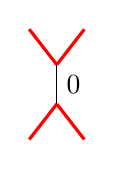
\begin{tikzpicture}[scale=0.5,baseline=(current bounding box.center)]
\draw[red,line width=0.4mm] (0,0) -- (-0.7,0.9);
\draw[red,line width=0.4mm] (0,0) -- (0.7,0.9);
\draw (0,0) to node[right] {$0$} (0,-1);
\draw[red,line width=0.4mm] (0,-1) -- (-0.7,-1.9);
\draw[red,line width=0.4mm] (0,-1) -- (0.7,-1.9);
%			\node at (0.8,1.1) {$*$};
%			\node at (-0.8,1.1) {$*$};
%			\node at (0.8,-2.1) {$*$};
%			\node at (-0.8,-2.1) {$*$};
\end{tikzpicture}
\end{equation*}
\noindent
can be realized in the framework of the $\Vec(\Z/2\Z)$ chain, we can study its action on the chain. For this purpose, we first need to change the basis using the identity
	\begin{equation}
		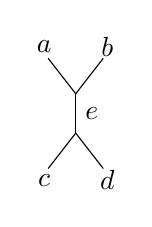
\begin{tikzpicture}[scale=0.5,baseline=(current bounding box.center)]
			\draw (0,0) -- (-0.7,0.9);
			\draw (0,0) -- (0.7,0.9);
			\draw (0,0) to node[right] {$e$} (0,-1);
			\draw (0,-1) -- (-0.7,-1.9);
			\draw (0,-1) -- (0.7,-1.9);
			\node at (0.8,1.2) {$b$};
			\node at (-0.8,1.2) {$a$};
			\node at (0.8,-2.2) {$d$};
			\node at (-0.8,-2.2) {$c$};
		\end{tikzpicture}=\sum_f\left(F_d^{abc}\right)_{ef}
		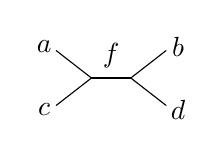
\begin{tikzpicture}[scale=0.5,baseline=(current bounding box.center)]
			\draw (0,0) -- (-0.9,0.7);
			\draw (0,0) -- (-0.9,-0.7);
			\draw (0,0) to node[above] {$f$} (1,0);
			\draw (1,0) -- (1.9,0.7);
			\draw (1,0) -- (1.9,-0.7);
			\node at (-1.2,0.8) {$a$};
			\node at (-1.2,-0.8) {$c$};
			\node at (2.2,0.8) {$b$};
			\node at (2.2,-0.8) {$d$};
		\end{tikzpicture}
	\end{equation}
which yields
	\begin{align}
		H&=-\sum \frac{1}{\sqrt{2}}\left(\left(F_*^{***}\right)_{00}
		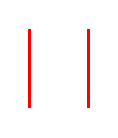
\begin{tikzpicture}[scale=0.5,baseline=(current bounding box.center)]
			\draw[red,line width=0.4mm] (0,0) -- (0,2);
			\draw[red,line width=0.4mm] (1.5,0) -- (1.5,2);
		\end{tikzpicture}+\left(F_*^{***}\right)_{01}
		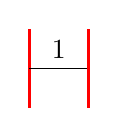
\begin{tikzpicture}[scale=0.5,baseline=(current bounding box.center)]
			\draw[red,line width=0.4mm] (0,0) -- (0,2);
			\draw (0,1) to node[above] {$1$} (1.5,1);
			\draw[red,line width=0.4mm] (1.5,0) -- (1.5,2);
		\end{tikzpicture}\ \right)\\
		&=-\sum\frac{1}{\sqrt{2}}\left(\ 
		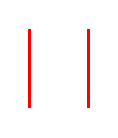
\begin{tikzpicture}[scale=0.5,baseline=(current bounding box.center)]
			\draw[red,line width=0.4mm] (0,0) -- (0,2);
			\draw[red,line width=0.4mm] (1.5,0) -- (1.5,2);
		\end{tikzpicture}+
		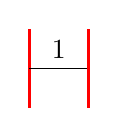
\begin{tikzpicture}[scale=0.5,baseline=(current bounding box.center)]
			\draw[red,line width=0.4mm] (0,0) -- (0,2);
			\draw (0,1) to node[above] {$1$} (1.5,1);
			\draw[red,line width=0.4mm] (1.5,0) -- (1.5,2);
		\end{tikzpicture}\ \right),
	\end{align}
where we have used the $F$-symbols we have computed above. 

The general Hilbert space of one site of the chain is $\mathbb{C}^2\oplus \mathbb{C}$ (see \eqref{eq:configs}), hence the space for three sites is
	\begin{align}\label{eq:hspaces}
		(\mathbb{C}^2\oplus \mathbb{C})\otimes(\mathbb{C}^2\oplus \mathbb{C})\otimes(\mathbb{C}^2\oplus \mathbb{C})=(\mathbb{C}^2\otimes\mathbb{C}\otimes\mathbb{C}^2)\oplus(\mathbb{C}\otimes\mathbb{C}^2\otimes\mathbb{C})\oplus\textrm{forbidden states},
	\end{align}
where forbidden states include, for example, those where all three objects are from the bimodule.
According to the right-hand side of \eqref{eq:hspaces}, valid local configurations of the chain are of the form
	\begin{equation*}
		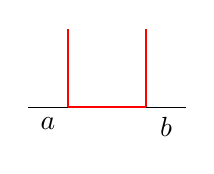
\begin{tikzpicture}[scale=1,baseline=(current bounding box.center)]
			\draw (-0.5,0) to node [below] {$a$} (0,0);
			\draw [red, line width=0.25mm] (0,0) -- (1,0);
			\draw (1,0) to node [below] {$b$} (1.5,0);
			\draw [red, line width=0.25mm] (0,0) -- (0,1);
			\draw [red, line width=0.25mm] (1,0) -- (1,1);
		\end{tikzpicture} \hspace{20pt}\text{and}\hspace{20pt}
		\begin{tikzpicture}[scale=1,baseline=(current bounding box.center)]
			\draw [red, line width=0.25mm] (-0.5,0) -- (0,0);
			\draw (0,0) to node [below] {$a$} (1,0);
			\draw [red, line width=0.25mm] (1,0) -- (1.5,0);
			\draw [red, line width=0.25mm] (0,0) -- (0,1);
			\draw [red, line width=0.25mm] (1,0) -- (1,1);
		\end{tikzpicture}
	\end{equation*}
\noindent
with $a,b\in\{0,1\}$. The local Hamiltonian 
	\begin{equation}
		h_i = -\frac{1}{\sqrt{2}}\left(\ 
		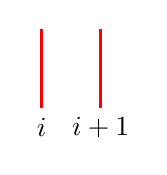
\begin{tikzpicture}[scale=0.5,baseline=(current bounding box.center)]
		\draw[red,line width=0.4mm] (0,0) -- (0,2);
		\draw[red,line width=0.4mm] (1.5,0) -- (1.5,2);
		\node at (0,-0.5) {$i$};
		\node at (1.5,-0.5) {$i+1$};
		\end{tikzpicture}+
		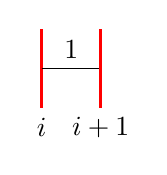
\begin{tikzpicture}[scale=0.5,baseline=(current bounding box.center)]
		\draw[red,line width=0.4mm] (0,0) -- (0,2);
		\draw (0,1) to node[above] {$1$} (1.5,1);
		\draw[red,line width=0.4mm] (1.5,0) -- (1.5,2);
		\node at (0,-0.5) {$i$};
		\node at (1.5,-0.5) {$i+1$};
		\end{tikzpicture}\ \right)
	\end{equation}
acts on these configurations in the following way: the first term of the Hamiltonian leaves the configurations invariant, while applying the second term yields
	\begin{align}\label{eq:action}
	\begin{split}
		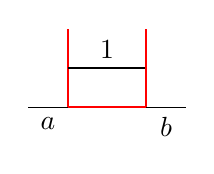
\begin{tikzpicture}[scale=1,baseline=(current bounding box.center)]
			\draw (-0.5,0) to node [below] {$a$} (0,0);
			\draw [red, line width=0.25mm] (0,0) -- (1,0);
			\draw (1,0) to node [below] {$b$} (1.5,0);
			\draw [red, line width=0.25mm] (0,0) -- (0,1);
			\draw (0,0.5) to node[above] {$1$} (1,0.5);
			\draw [red, line width=0.25mm] (1,0) -- (1,1);
		\end{tikzpicture}&=
		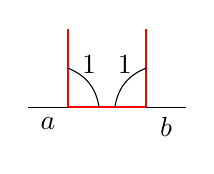
\begin{tikzpicture}[scale=1,baseline=(current bounding box.center)]
			\draw (-0.5,0) to node [below] {$a$} (0,0);
			\draw [red, line width=0.25mm] (0,0) -- (1,0);
			\draw (1,0) to node [below] {$b$} (1.5,0);
			\draw [red, line width=0.25mm] (0,0) -- (0,1);
			\draw [red, line width=0.25mm] (1,0) -- (1,1);
			\draw (0,0.5) to[bend left] node[above] {$1$} (0.4,0);
			\draw (1,0.5) to[bend right] node[above] {$1$} (0.6,0);
		\end{tikzpicture}\\
		&=(-1)^{a+b}
		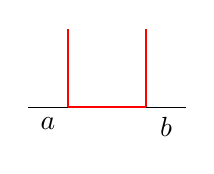
\begin{tikzpicture}[scale=1,baseline=(current bounding box.center)]
			\draw (-0.5,0) to node [below] {$a$} (0,0);
			\draw [red, line width=0.25mm] (0,0) -- (1,0);
			\draw (1,0) to node [below] {$b$} (1.5,0);
			\draw [red, line width=0.25mm] (0,0) -- (0,1);
			\draw [red, line width=0.25mm] (1,0) -- (1,1);
		\end{tikzpicture}\equiv Z_a\otimes Z_b
		\end{split}
		\\\label{eq:action2}
		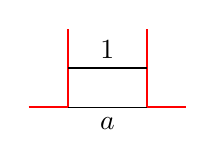
\begin{tikzpicture}[scale=1,baseline=(current bounding box.center)]
			\draw [red, line width=0.25mm] (-0.5,0) -- (0,0);
			\draw (0,0) to node[below] {$a$} (1,0);
			\draw [red, line width=0.25mm] (1,0) -- (1.5,0);
			\draw [red, line width=0.25mm] (0,0) -- (0,1);
			\draw [red, line width=0.25mm] (1,0) -- (1,1);
			\draw (0,0.5) to node[above] {$1$} (1,0.5);
		\end{tikzpicture}&=
		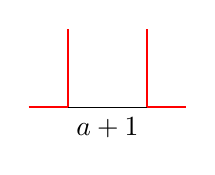
\begin{tikzpicture}[scale=1,baseline=(current bounding box.center)]
			\draw [red, line width=0.25mm] (-0.5,0) -- (0,0);
			\draw (0,0) to node[below] {$a+1$} (1,0);
			\draw [red, line width=0.25mm] (1,0) -- (1.5,0);
			\draw [red, line width=0.25mm] (0,0) -- (0,1);
			\draw [red, line width=0.25mm] (1,0) -- (1,1);
		\end{tikzpicture}\equiv X_a
	\end{align}
A general basis state that lives in $(\mathbb{C}^2\oplus \mathbb{C})\otimes(\mathbb{C}^2\oplus \mathbb{C})\otimes(\mathbb{C}^2\oplus \mathbb{C})$ is of the form
	\begin{equation}
		\lvert x_{i-1}, x_i, x_{i+1}\rangle=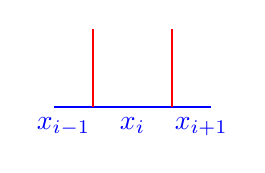
\begin{tikzpicture}[scale=1,baseline=(current bounding box.center)]
		\draw [blue, line width=0.25mm] (-0.5,0) to node[below, near start] {$x_{i-1}$} (0,0);
		\draw [blue, line width=0.25mm] (0,0) to node[below] {$x_i$} (1,0);
		\draw [blue, line width=0.25mm] (1,0) to node[below, near end] {$x_{i+1}$} (1.5,0);
		\draw [red, line width=0.25mm] (0,0) -- (0,1);
		\draw [red, line width=0.25mm] (1,0) -- (1,1);
		\end{tikzpicture}
	\end{equation}
with $x_{i-1}, x_i, x_{i+1}\in\{0,1,*\}$. The goal is now to find an operator that acts on this basis that gives exactly what we have derived in \eqref{eq:action} and \eqref{eq:action2}, which means we want an expression of $h_i$ of the form
	\begin{equation}
		h_i\lvert x_{i-1},x_i,x_{i+1}\rangle=-\frac{1}{\sqrt{2}}\left(\mathbb{I}+A\right)\lvert x_{i-1},x_i,x_{i+1}\rangle
	\end{equation}
with some operator $A$. Note that we do not need to worry about how it acts on forbidden state, e.g.\ $\lvert *,*,*\rangle$. Since there are two possible configurations, we distinguish between these two cases:
	\begin{enumerate}
		\item When $x_i=*$, we are in the case of $\eqref{eq:action}$, which means the object in the middle is projected onto the state $\lvert*\rangle\langle*\rvert$. A Pauli-$Z$ operator acts on the objects $x_{i-1}$ and $x_{i+1}$, but only on the $\mathbb{C}^2$-part of the Hilbert space. Hence, we additionally need an operator that acts on $\mathbb{C}$, but since we projected the site $i$ onto $\lvert *\rangle$, and any states of the form $\lvert *,*,\cdot\rangle$ and $\lvert \cdot,*,*\rangle$ are forbidden anyway, it does not matter which operator we put here and we just denote it $\hat{O}$ \footnote{We can pick $\hat{O}=0$ for simplicity.}. Following these arguments, the resulting expression for the operator $A$ is
			\begin{equation}
				A=(Z\oplus\hat{O})\otimes\lvert*\rangle\langle*\rvert\otimes(Z\oplus\hat{O}).
			\end{equation}
		\item When $x_{i-1}=x_{i+1}=*$, the outer sited are projected onto $\lvert*\rangle\langle*\rvert$ and as we have seen in \eqref{eq:action2}, the Hamiltonian acts as a Pauli-$X$ operator on the middle site. For the same reasons as above, we add the operator $\hat{O}$ and get
			\begin{equation}
				A=\lvert*\rangle\langle*\rvert\otimes(X\oplus\hat{O})\otimes\lvert*\rangle\langle*\rvert.
			\end{equation}
	\end{enumerate}
The resulting local Hamiltonian is
	\begin{equation}
	\begin{split}
	h_i=&-\frac{1}{\sqrt{2}}\left(\mathbb{I}+(Z\oplus\hat{O})\otimes\lvert*\rangle\langle*\rvert\otimes(Z\oplus\hat{O})\right.\\&\left.+\lvert*\rangle\langle*\rvert\otimes(X\oplus\hat{O})\otimes\lvert*\rangle\langle*\rvert\right).
	\end{split}
	\end{equation}
If we fix some edge, e.g.\ the boundaries, to $*$ we restrict ourselves to states of the form
	\begin{figure}[H]
		\centering
		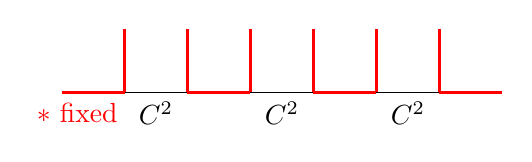
\begin{tikzpicture}[scale=0.8,baseline=(current bounding box.center)]
		\draw[red,line width=0.4mm] (0.5,0) to node[below,near start] {$*$ fixed} (1.5,0);
		\draw[red,line width=0.4mm] (1.5,0) -- (1.5,1);
		\draw[black] (1.5,0) to node [below] {$\mathbb{C}^2$} (2.5,0);
		\draw[red,line width=0.4mm] (2.5,0) -- (2.5,1);
		\draw[red,line width=0.4mm] (2.5,0) -- (3.5,0);
		\draw[red,line width=0.4mm] (3.5,0) -- (3.5,1);
		\draw[black] (3.5,0) to node [below] {$\mathbb{C}^2$} (4.5,0);
		\draw[red,line width=0.4mm] (4.5,0) -- (4.5,1);
		\draw[red,line width=0.4mm] (4.5,0) -- (5.5,0);
		\draw[red,line width=0.4mm] (5.5,0) -- (5.5,1);
		\draw[black] (5.5,0) to node [below] {$\mathbb{C}^2$} (6.5,0);
		\draw[red,line width=0.4mm] (6.5,0) -- (6.5,1);
		\draw[red,line width=0.4mm] (6.5,0) -- (7.5,0);
		\end{tikzpicture},
	\end{figure}
\noindent
so we effectively have a system of qubits
	\begin{figure}[H]
		\centering
		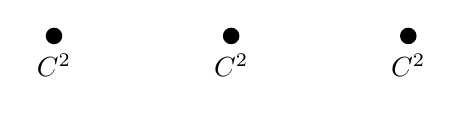
\begin{tikzpicture}[scale=1.5,baseline=(current bounding box.center)]
		\fill[black] (0,0) circle (0.07cm);
		\node at (0,-0.25) {$\mathbb{C}^2$};
		\fill[black] (1.5,0) circle (0.07cm);
		\node at (1.5,-0.25) {$\mathbb{C}^2$};
		\fill[black] (3,0) circle (0.07cm);
		\node at (3,-0.25) {$\mathbb{C}^2$};
		\end{tikzpicture}.
	\end{figure}
\noindent
On this Hilbert space, the effective Hamiltonian is 
	\begin{equation}\label{eq:eff}
		H_\mathrm{effective}=-\frac{1}{\sqrt{2}}\sum_{i\in\text{half chain}}\mathbb{I}+Z_iZ_{i+1}+X_i,
	\end{equation}
which is the Hamiltonian that corresponds to the transverse Ising model. The other possibility is to fix the boundaries to $\mathbb{C}^2$, in which case we have states of the form
	\begin{figure}[H]
		\centering
		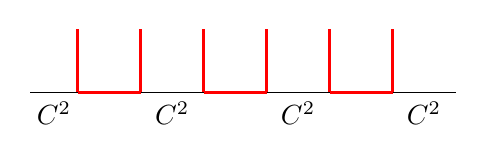
\begin{tikzpicture}[scale=0.8]
		\draw[black] (-0.25,0) to node [below] {$\mathbb{C}^2$} (0.5,0);
		\draw[red,line width=0.4mm] (0.5,0) -- (0.5,1);
		\draw[red,line width=0.4mm] (0.5,0) -- (1.5,0);
		\draw[red,line width=0.4mm] (1.5,0) -- (1.5,1);
		\draw[black] (1.5,0) to node [below] {$\mathbb{C}^2$} (2.5,0);
		\draw[red,line width=0.4mm] (2.5,0) -- (2.5,1);
		\draw[red,line width=0.4mm] (2.5,0) -- (3.5,0);
		\draw[red,line width=0.4mm] (3.5,0) -- (3.5,1);
		\draw[black] (3.5,0) to node [below] {$\mathbb{C}^2$} (4.5,0);
		\draw[red,line width=0.4mm] (4.5,0) -- (4.5,1);
		\draw[red,line width=0.4mm] (4.5,0) -- (5.5,0);
		\draw[red,line width=0.4mm] (5.5,0) -- (5.5,1);
		\draw[black] (5.5,0) to node [below] {$\mathbb{C}^2$} (6.5,0);
		\end{tikzpicture}.
	\end{figure}
\noindent
The effective Hamiltonian for these states is also of the form \eqref{eq:eff}. Hence, if we do not fix any boundaries, we get the direct sum of two copies of Ising.